\documentclass{shortart}

\usepackage{amsmath, amssymb, amsthm}
\usepackage{todonotes}
\usepackage{tikz}
\usepackage{booktabs}

\title{The Lemniscate Sine}
\author{Dexter Chua}

\tikzset{circ/.style = {fill, circle, inner sep = 0, minimum size = 3}}

\newtheorem*{prop}{Proposition}
\newtheorem*{thm}{Theorem}

\theoremstyle{definition}
\newtheorem*{defi}{Definition}
\newtheorem*{eg}{Example}

\newcommand\A{\mathbb{A}}
\newcommand\C{\mathbb{C}}
\newcommand\R{\mathbb{R}}
\newcommand\Z{\mathbb{Z}}
\newcommand\Q{\mathbb{Q}}
\newcommand\Cl{\mathrm{Cl}}
\renewcommand\P{\mathbb{P}}
\renewcommand\d{\mathrm{d}}
\let\sl\relax
\DeclareMathOperator\sl{sl}

\begin{document}
%\section{Introduction}
%Starting with the trigonometric sine function, we enter the world of elliptic integrals, and study the lemniscate sine in detail. We shall do very explicit and elementary calculations, but will interpret the results in the modern language of Riemann surfaces and, in particular, elliptic curves. At the end, we will use the explicit calculations to compute ray class fields using the theory of complex multiplication.

\section{Sine}
The sine function, as we learnt in high school, is closely related to the arc length of the circle. We will describe this in a slightly funny way. Consider the circle of unit diameter with center $(0, \frac{1}{2})$:
\begin{center}
  \begin{tikzpicture}
    \draw (-4, 0) -- (4, 0) node [right] {$x$};
    \draw (0, -0.5) -- (0, 3.5) node [above] {$y$};

    \draw [blue, semithick] (0, 1.5) circle [radius=1.5];

    \draw (0, 0) -- (0.75, 2.799) node [pos=0.5, left] {$r$};
    \draw (0.3, 0) arc(0:75:0.3) node [right] {\;\,$\theta$};
  \end{tikzpicture}
\end{center}
By some elementary geometry, we find that $r = \sin \theta$. The arc length $s$ is given by
\[
  (\d s)^2 = (\d r)^2 + (r \;\d \theta)^2.
\]
We have
\[
  \d \theta = \frac{\d r}{\cos \theta} = \frac{\d r}{\sqrt{1 - \sin^2 \theta}} = \frac{\d r}{\sqrt{1 - r^2}}.
\]
So we can write the line element as
\[
  \d s = \frac{1}{\sqrt{1 - r^2}}\;\d r
\]
Thus, the arc length function is given
\[
  s(r_0) = \int_0^{r_0} \frac{1}{\sqrt{1 - r^2}}\;\d r.
\]
This is, of course, the familiar arcsine function, inverse to the even more familiar sine function.

Note that here we have a square root sitting inside the integrand. For the arc length function, we simply always take the positive square root. However, if we want to extend arcsine and sine to \emph{complex} functions by replacing the integral with a contour integral, then we cannot always stick with the above choice.

The solution is to instead think about the Riemann surface of the function $\frac{1}{\sqrt{1 - r^2}}$, which is given by the circle $r^2 + t^2 = 1$:
\begin{center}
  \begin{tikzpicture}
    \draw (-2, 0) -- (2, 0) node [right] {$r$};
    \draw (0, -2) -- (0, 2) node [above] {$t$};

    \draw [red, semithick] circle [radius=1.3];
  \end{tikzpicture}
\end{center}
We can then write the integral as
\[
  s(z) = \int_0^z \frac{\d r}{t},
\]
where $z$ is now viewed as a point in $R = \{(r, t) \in \C^2: r^2 + t^2 = 1\}$. This integral depends not only on $z$, but also on the path taken from $0$ to $z$. In general, it is well-defined only up to a \emph{period}, namely the integral of $\frac{\d r}{t}$ around a closed loop. Thus, the inverse function, namely sine, is a singly-periodic function.

It is important to note that this circle is \emph{different} from the previous circle. When we discuss the Lemniscate sine soon, we will work with two rather different shapes.

Before we end the section, note that to study the sine function, which is a function defined on $R$, it is often convenient to pick an isomorphism between $R$ and $\P^1$ given by stereographic projection.
\begin{center}
  \begin{tikzpicture}[scale=0.65]
    \draw [red, semithick] circle [radius=2];
    \draw (-5.5, 0) -- (5.5, 0);
    \draw (0, 2) node [circ] {};
    \node at (1.414, 1.414) [anchor = south west] {$(r, t)$};
    \node at (1.414, 1.414) [circ] {};
    \draw (0, 2) -- (4.8259, 0) node [circ] {} node [above] {$u$};
    \draw (0, -3) -- (0, 3);
  \end{tikzpicture}
\end{center}
This is given by the formulae
\[
  r = \frac{2u}{1 + u^2},\quad t = \frac{1 - u^2}{1 + u^2}
\]
Substituting in, we find
\[
  \frac{\d r}{\sqrt{1 - r^2}} = \frac{1}{\sqrt{1 - \big(\frac{2u}{1 + u^2}\big)^2}} \cdot \frac{2 (1 + u^2) - 4u^2}{(1 + u^2)^2}\;\d u = \frac{1 + u^2}{1 - u^2} \cdot \frac{2 (1 - u^2)}{(1 + u^2)^2}\;\d u = \frac{2\;\d u}{1 + u^2},
\]
which is the integral of a nice, rational function.

\section{The Lemniscate Sine}
The \emph{lemniscate sine} is an example of an elliptic integral. Elliptic integrals first arose when people studied problems analogous to the above but for ellipses, and integrals that looked similar were called elliptic integrals. We shall not be interested in ellipses here, because they are less interesting. Fix two foci $F_{\pm} = (\pm a, 0) \in \R^2$, and consider the locus of all points $P = (x, y)$ such that
\[
  \|P - F_+\| \cdot \|P - F_-\| = \|0 - F_+\| \cdot \|0 - F_-\|.
\]
\begin{center}
  \begin{tikzpicture}
    \draw [blue, semithick, domain=-40:40, variable=\t] plot ({2.5 * sqrt(sqrt(abs(2 * cos (2 * \t)))) * cos (\t)}, {2.5 * sqrt(sqrt(abs(2 * cos (2 * \t)))) * sin (\t)});
    \draw [blue, semithick, domain=45:40, variable=\t, samples=50] plot ({2.5 * sqrt(sqrt(abs(2 * cos (2 * \t)))) * cos (\t)}, {2.5 * sqrt(sqrt(abs(2 * cos (2 * \t)))) * sin (\t)});
    \draw [blue, semithick, domain=-45:-40, variable=\t, samples=50] plot ({2.5 * sqrt(sqrt(abs(2 * cos (2 * \t)))) * cos (\t)}, {2.5 * sqrt(sqrt(abs(2 * cos (2 * \t)))) * sin (\t)});

    \draw [blue, semithick, domain=140:220, variable=\t] plot ({2.5 * sqrt(sqrt(abs(2 * cos (2 * \t)))) * cos (\t)}, {2.5 * sqrt(sqrt(abs(2 * cos (2 * \t)))) * sin (\t)});
    \draw [blue, semithick, domain=135:140, variable=\t, samples=50] plot ({2.5 * sqrt(sqrt(abs(2 * cos (2 * \t)))) * cos (\t)}, {2.5 * sqrt(sqrt(abs(2 * cos (2 * \t)))) * sin (\t)});
    \draw [blue, semithick, domain=225:220, variable=\t, samples=50] plot ({2.5 * sqrt(sqrt(abs(2 * cos (2 * \t)))) * cos (\t)}, {2.5 * sqrt(sqrt(abs(2 * cos (2 * \t)))) * sin (\t)});
    \draw (-4, 0) -- (4, 0) node [right] {$x$};
    \draw (0, -2) -- (0, 2) node [above] {$y$};
    \draw (0, 0) -- (2.1651, 1.25) node [pos=0.5, above] {$r$};

    \draw (0.5, 0) arc(0:30:0.5) node [pos=0.7, right] {$\theta$};
  \end{tikzpicture}
\end{center}
Explicitly, this is given by
\[
  ((x - a)^2 + y^2)((x + a)^2 + y^2) = a^4.
\]
Equivalently, this is
\[
  (x^2 + y^2)^2 = 2a^2 (x^2 - y^2).
\]

It is convenient to set $a = \frac{1}{\sqrt{2}}$, and using polar coordinates, this equation becomes
\[
  r^2 = \cos 2\theta.
\]
We then have
\[
  \d \theta = \frac{-r}{\sin 2\theta}\;\d r = \frac{-r}{\sqrt{1 - r^4}}\;\d r.
\]
Thus, the line element is
\[
  \d s = \frac{1}{\sqrt{1 - r^4}}\;\d r,
\]
and we have a lemniscate arcsine
\[
  s(r_0) = \int_0^{r_0} \frac{1}{\sqrt{1 - r^4}}\;\d r
\]
with inverse $\sl(s)$. Again, we want to promote this to a complex function. From now on, we will replace $r$ with $x$, since explicit coordinates for the lemniscate itself will not be of much use. Then the associated Riemann surface is given by
\[
  R = \{(x, y) \in \C^2: y^2 = 1 - x^4\}.
\]
Then
\[
  s = \int \frac{\d x}{y}.
\]
Observe that this surface is singular at infinity. Which is bad. However, we can blow this up at infinity to resolve the singularity, and since we are working with curves, any rational map is automatically a morphism, and so we don't have to think about infinity much.

A key observation is that projection onto the $x$ coordinate exhibits $R$ as a double cover of $\P^1$ branched at four points (it cannot be branched at infinity since there is always an even number of branch points), and so by Riemann-Hurwitz, $R$ is a torus. This means $R$ admits a holomorphic and non-vanishing differential, and one can check $\frac{\d x}{y}$ is one.

Since $R$ is topologically a torus, its homology is generated by two loops, and $s$ will be defined up to the integrals of those loops, which we expect to be an integer lattice $\Lambda$ in $\C$. We will explicitly identify this lattice soon. What this means is that $s$ actually gives an explicit identification $R \overset{\sim}{\to} \C/\Lambda$. Surjectivity is automatic, and injectivity is given by the Abel--Jacobi theorem, since if $s(p) = s(p')$, then $p - p'$ is killed by the Abel--Jacobi map, and hence $p \sim p'$. This is possible only if $p = p'$ as $R$ is not $\P^1$.

To understand the lattice, we pick two generated loops as follows:
\begin{center}
  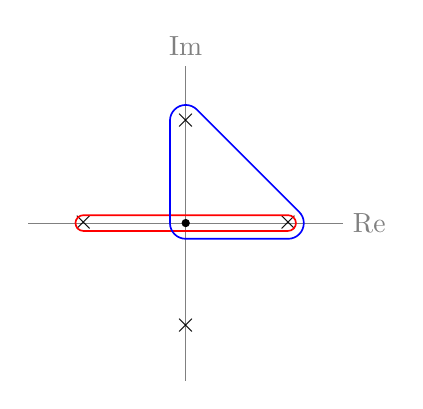
\begin{tikzpicture}
    \draw [gray] (-2, 0) -- (2, 0) node [right] {$\mathrm{Re}$};
    \draw [gray] (0, -2) -- (0, 2) node [above] {$\mathrm{Im}$};

    \node at (0, 1.3) {$\times$};
    \node at (0, -1.3) {$\times$};
    \node at (1.3, 0) {$\times$};
    \node at (-1.3, 0) {$\times$};

    \node [circ] at (0, 0) {};

    \draw [red, semithick] (0, -0.1) -- (1.3, -0.1) arc(-90:90:0.1) -- (-1.3, 0.1) arc(90:270:0.1) -- (0, -0.1);

    \draw [blue, semithick] (0, -0.2) -- (1.3, -0.2) arc(-90:45:0.2) -- (0.1414, 1.4414) arc(45:180:0.2) -- (-0.2, 0) arc(180:270:0.2);
  \end{tikzpicture}
\end{center}
The horizontal loop has a very geometric interpretation, since the path lies entirely within the real axis. Indeed, this just corresponds to integrating the line element along the whole lemniscate, and the integral is just the total arc length of the lemniscate, $2\Omega$. It is written this way so that the length of half of the lemniscate is $\Omega$, which is exactly the contribution we get if we go around the branch point at $1$ and then return to the ``origin'' (of course, on the Riemann surface, this is a distinct point that the origin, as it is on the other sheet).

It remains to understand what happens when we go around the branch point at $i$. This follows from the simple observation that the integrand is invariant under $x \mapsto ix$, while $\d x$ gets multiplied by $i$ under this operation. So we find that
\[
  s(iz) = i s(z).
\]
So it follows that the other homology class has an integral of $(1 + i)\Omega$. Thus,
\[
  \Lambda = \langle 2\Omega, (1 + i)\Omega\rangle.
\]
The inverse function $\sl$ is then a double periodic function with period lattice $\Lambda$ with zeroes given by $\Lambda \cup (\Omega + \Lambda)$.
\section{Complex Multiplication}
We have already observed above that
\[
  \sl(iz) = i \sl(z).
\]
We can think of this as follows --- we fix $O = (0, 1)$ as our basepoint of $R$, which corresponds to the point $0 \in \C/\Lambda$. Then multiplication by $i$ is an automorphism of $\C/\Lambda$, which should then descend to an automorphism of $R$. This formula gives a very concrete description of what the induced map on $R$ is --- it is simply multiplication by $i$ in the $x$ coordinates!

We might hope that there are more formulas of this sort. For example, an addition formula like
\[
  \sin(z + w) = \sin z \sqrt{1 - \sin^2 w} + \sin w \sqrt{1 - \sin^2 z}
\]
would be helpful. To look for such formulae, we may try playing around with some substitutions and see what we get. Previously, for the circle, we had the substitution $x = \frac{2u}{1 + u^2}$ that turned things into rational functions. We might try a similar substitution. If we want $1 - x^4$ to become a perfect square and we can get rid of the radical, we should set
\[
  x^2 = \frac{2u^2}{1 + u^4}.
\]
Doing the substitution yields
\[
  \frac{\d x}{\sqrt{1 - x^4}} = \frac{1 + u^4}{1 - u^4} \cdot \frac{4u(1 - u^4)}{(1 + u^4)^2} \cdot \frac{\d u}{2x} = \frac{\sqrt{2}\;\d u}{\sqrt{1 + u^4}}
\]
This looks quite like what we originally had, except for the change in sign below. Thus, we put $u = \zeta_8 v$, and then we get
\[
  \frac{\d x}{\sqrt{1 - x^4}} = \frac{(1 + i)\;\d v}{\sqrt{1 + v^4}}.
\]
Integrating and putting in the right bounds, we find that
\[
  s\left(\frac{(1 + i) v_0}{\sqrt{1 - v_0^4}}\right) = (1 + i) s(v_0).
\]
In other words, we have
\[
  \sl((1 + i)z) = \frac{(1 + i) \sl(z)}{\sqrt{1 - \sl(z)^4}}.
\]
Taking complex conjugates, we get
\[
  \sl((1 - i)z) = \frac{(1 - i) \sl(z)}{\sqrt{1 - \sl(z)^4}}.
\]
Crucially, since $(1 + i)(1 - i) = 2$, we can iterate these two formulas to obtain
\[
  \sl(2z) = \frac{2\sl(z)\sqrt{1 - \sl(z)^4}}{1 + \sl(z)^4}.
\]
The presence of these $\sqrt{1 - \sl(z)^4}$ may be a bit off-putting, but there is no reason to fear them --- they are simply the $y$ coordinates of $R$, which we should think of as the lemniscate arcsine of $z$. The ambiguity in sign is fixed by what happens in a small neighbourhood of $2$, where we choose $\sqrt{1 - \sl(z)^4}$ to be positive whenever $z$ is small and positive.

It is an elementary exercise to iterate these formulas to obtain
\begin{align*}
  \sl(2(1 + i)z) &= \frac{2(1 + i) \sl(z) \sqrt{1 - \sl(z)^4} (1 + \sl(z)^4)}{1 - 6 \sl(z)^4 + \sl(z)^8}\\
  \sl(4z) &= \frac{4\sl(z) \sqrt{1 - \sl(z)^4} (1 + \sl(z)^4) (1 - 6 \sl(z)^4 + \sl(z)^8)}{1 + 20 \sl(z)^4 - 26 \sl(z)^8 + 20 \sl(z)^{12} + \sl(z)^{16}}
\end{align*}

Given the duplication formula for $\sl(2z)$, it is reasonable to guess that we might have an addition formula of the form
\[
  \sl(z + w) = \frac{\sl(z) \sqrt{1 - \sl(w)^4} + \sl(w) \sqrt{1 - \sl(z)^4}}{1 + \sl(z)^2 \sl(w)^2},
\]
from which we can deduce all the above formulae using that $\sl(iz) = i \sl(z)$.

A poor man's way of proving the formula would be to set $w = c - z$ for some constant $c$, and then differentiate the right-hand side to see it is constant. There are more modern ways of doing so, but is out of the scope of this discussion.

We should think of this formula as transporting the obvious addition structure on $\C/\Lambda$ to give an addition rule on $R$.
\section{Torsion Points}
The duplication formulae above allow us to consider the $(1 + i)^n$-torsion points of $R$, i.e.\ the points such that acting by $(1 + i)^n$ sends the point back to the origin. There is a slight subtlety here, due do the fact that we are working with $\sl$, which is the composition $\C/\Lambda \to R \overset{\pi}{\to} \P^1$. If $\sl(z) = 0$, then the corresponding point in $R$ need not be the origin. It could be the other point $(0, -1)$. Fortunately, we already know exactly which point gets mapped to $(0, -1)$, namely $\Omega$, which is the unique $(1 + i)$-torsion point of $\C/\Lambda$.

We might also worry about the two points at infinity, which is not adequately captured by our formula. Observing that
\[
  \sl((1 + i)z) = \frac{(1 + i)\sl(z)}{\sqrt{1 - \sl(z)^4}},
\]
and the fact that $\sl(\frac{\Omega}{2}) = 1$, we know that the two points at infinity are $\frac{1 \pm i}{2} \Omega$, which are the remaining $2$-torsion points. These let us conclude

\begin{prop}
  $\sl((1 + i)^n z) = \infty$ iff $z$ is a $(1 + i)^{n + 2}$-torsion point but not an $(1 + i)^{n + 1}$-torsion point.
\end{prop}
This lets us compute the higher torsion points:
\begin{center}
  \begin{tabular}{cl}
    \toprule
    $n$ & $(1 + i)^n$-torsion points\\
    \midrule
    0 & $(0, 1)$\\
    1 & $(0, -1)$\\
    2 & $\infty, \infty$ \\
    3 & $(\pm 1, 0), (\pm i, 0)$\\
    4 & $(\zeta_8^k, \pm \sqrt{2})$ \hfill $k = 1, 3, 5, 7$ \\
    5 & $(i^k \sqrt[4]{3 \pm_a 2 \sqrt{2}}, \pm_b \sqrt{2 \mp_a 2\sqrt{2}})$\quad\quad $k = 0, 1, 2, 3$\\
    \bottomrule
  \end{tabular}
\end{center}
Finding higher-order torsion points will require advanced WolframAlpha techniques.

Recall that we can find ray class fields of $Q(i)$ by adjoining the torsion points of the curve with CM by $Q(i)$. We need to first identify a Weber function, which is given by quotienting out $R$ by the automorphism group. The automorphism group multiplies by powers of $i$, and so we find that $h(x, y) = y$ is a perfectly good Weber function on $R$. So we find that
\begin{enumerate}
  \item The ray class field modulo $(1 + i)^3$ is still just $\Q(i)$.
  \item The ray class field modulo $(1 + i)^4 = (4)$ is $\Q(i, \sqrt{2})$.
  \item The ray class field modulo $(1 + i)^5$ is $\Q(i, \sqrt{2 + 2 \sqrt{2}})$.
\end{enumerate}
We can compute the ray class groups explicitly, using the definition of the ray class group, and see that they match. Observe that since $\Q(i)$ has class number $1$, we we can decompose
\[
  \A_{\Q(i)}^\times = \frac{\Q(i)^\times}{\mu_4} \times \C^\times \times \prod_{v \nmid \infty} \mathcal{O}_v^\times,
\]
and so
\[
  C_{\Q(i)} = \frac{\C^\times \times \prod_{v \nmid \infty} \mathcal{O}_v^\times}{\mu_4}.
\]
The ray class group modulo $\mathfrak{m} = (1 + i)^k$ is then given by
\[
  \Cl_\mathfrak{m} = \frac{\mathcal{O}_{(1 + i)}^\times}{\mu_4 \times (1 + (1 + i)^k \mathcal{O}_{(1 + i)})} = \left(\frac{\Z[i]}{(1 + i)^k}\right)^\times \Big/ \mu_4.
\]
The invertible elements in $\Z[i]/(1 + i)^k$ are exactly those $(1 + i)$ does not divide, i.e.\ those with odd norm. Thus, we see that
\[
  \Cl_{(1 + i)^3} = 0,\quad \Cl_{(1 + i)^4} = C_2,\quad \Cl_{(1 + i)^5} = C_2 \times C_2,
\]
in agreement with above (exercise: find the other subfields on $\Q(i, \sqrt{2 + 2\sqrt{2}})$).
\end{document}
